	\section{Regression Methods}
	Conventional regression models are estimated using the ordinary
	least squares (OLS) technique, and are referred to as `Model I
	regression'\citep{CornCoch,ludbrook97}. A key feature of Model I
	models is that the independent variable is assumed to be measured
	without error. As often pointed out in several papers
	\citep{BA83,ludbrook97}, this assumption invalidates simple linear
	regression for use in method comparison studies, as both methods
	must be assumed to be measured with error.
	
	The use of regression models that assumes the presence of error in
	both variables $X$ and $Y$ have been proposed for use instead.
	\citep{CornCoch,ludbrook97}, These methodologies are collectively
	known as `Model II regression'. They differ in the method used to
	estimate the parameters of the regression.
	
	Regression estimates depend on formulation of the model. A
	formulation with one method considered as the $X$ variable will
	yield different estimates for a formulation where it is the $Y$
	variable. With Model I regression,the models fitted in both cases
	will entirely different and inconsistent. However with Model II
	regression, they will be consistent and complementary.
	
	\subsection{Deming's Regression}
	The most commonly known Model II methodology is known as Deming's
	Regression, (also known an Ordinary Least Product regression).
	Deming regression is recommended by \citet*{CornCoch} as the
	preferred Model II regression for use in method comparison
	studies. As previously noted, the Bland Altman Plot is
	uninformative about the comparative influence of proportional bias
	and fixed bias. Deming's regression provides independent tests for
	both types of bias.
	
	For a given $\lambda$, \citet{Kummel} derived the following
	estimate for the Demimg regression slope parameter. ($\alpha$ is
	simply estimated by using the identity
	$\bar{Y}-\hat{\beta}\bar{X}$.)
	\begin{equation}
	\hat{\beta} =\quad \frac{S_{YY} - \lambda S_{XX}+[(S_{YY} -
		\lambda S_{XX})^{2}+ 4\lambda S^{2}_{XY}]^{1/2}}{2S_{XY}}
	\end{equation}
	
	
	As with conventional regression methodologies, Deming's regression
	calculates an estimate for both the slope and intercept for the
	fitted line, and standard errors thereof. Therefore there is
	sufficient information to carry out hypothesis tests on both
	estimates, that are informative about presence of fixed and
	proportional bias.
	
	A $95\%$ confidence interval for the intercept estimate can be
	used to test the intercept, and hence fixed bias, is equal to
	zero. This hypothesis is accepted if the confidence interval for
	the estimate contains the value $0$ in its range. Should this be,
	it can be concluded that fixed bias is not present. Conversely, if
	the hypothesis is rejected, then it is concluded that the
	intercept is non zero, and that fixed bias is present.
	
	Testing for proportional bias is a very similar procedure. The
	$95\%$ confidence interval for the slope estimate can be used to
	test the hypothesis that the slope is equal to $1$. This
	hypothesis is accepted if the confidence interval for the estimate
	contains the value $1$ in its range. If the hypothesis is
	rejected, then it is concluded that the slope is significant
	different from $1$ and that a proportional bias exists.
	
	For convenience, a new data set shall be introduced to demonstrate
	Demings regression. Measurements of transmitral volumetric flow
	(MF) by doppler echocardiography, and left ventricular stroke
	volume (SV) by cross sectional echocardiography in 21 patients
	withour aortic valve disease are tabulated in \citet{zhang}. This
	data set features in the discussion of method comparison studies
	in \citet[p.398]{images/AltmanBook} .
	
	\newpage
	% latex table generated in R 2.6.0 by xtable 1.5-5 package
	% Tue Sep 01 13:31:17 2009
	\begin{table}[h!]
		\begin{center}
			\begin{tabular}{|c|c|c||c|c|c||c|c|c|}
				\hline
				Patient & MF  & SV  & Patient & MF  & SV  & Patient & MF  & SV \\
				&($cm^{3}$)&  ($cm^{3}$) & &($cm^{3}$)&  ($cm^{3}$) & &($cm^{3}$)&  ($cm^{3}$)
				\\
				\hline
				1 & 47 & 43 &  8 & 75 & 72 &  15 & 90 & 82 \\
				2 & 66 & 70 & 9 & 79 & 92 &  16 & 100 & 100 \\
				3 & 68 & 72 & 10 & 81 & 76 & 17 & 104 & 94 \\
				4 & 69 & 81 & 11 & 85 & 85 &  18 & 105 & 98 \\
				5 & 70 & 60 & 12 & 87 & 82 & 19 & 112 & 108 \\
				6 & 70 & 67 & 13 & 87 & 90 & 20 & 120 & 131 \\
				7 & 73 & 72 & 14 & 87 & 96 &  21 & 132 & 131 \\
				
				\hline
			\end{tabular}
			\caption{Transmitral volumetric flow(MF) and left ventricular
				stroke volume (SV) in 21 patients. (Zhang et al 1986)}
		\end{center}
	\end{table}
	\newpage
	\begin{figure}[h!]
		% Requires \usepackage{graphicx}
		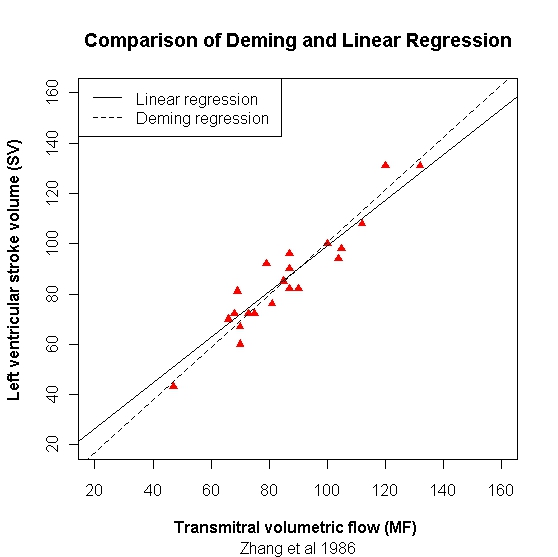
\includegraphics[width=130mm]{images/ZhangDeming.jpeg}
		\caption{Deming Regression For Zhang's Data}\label{ZhangDeming}
	\end{figure}
	
	Deming's Regression suffers from some crucial drawback. Firstly it
	is computationally complex, and it requires specific software
	packages to perform calculations.Secondly it is uninformative
	about the comparative precision of two methods of measurement.
	Most importantly \citet{CarollRupert} states that Deming's
	regression is acceptable only when the precision ratio ($\lambda$,
	in their paper as $\eta$) is correctly specified ,but in practice
	this is often not the case, with the $\lambda$ being
	underestimated.
	\newpage
	%%%%%%%%%%%%%%%%%%%%%%%%%%%%%%%%%%%%%%%%%%%%%%%%%%%%%%%%%%%%%%%%%%%%%%%%%%%%%%%%%%%%%%%%%%%%%%%%%%%%%%%%%%%%%%%%%%
	
	

\section*{Deming Regression}

Performance of Deming regression analysis in case of misspecified analytical error ratio in method comparison studies

%-----------------------------------------------------------------------------------------------%
Application of Deming regression analysis to interpret method comparison data presupposes specification of the 
squared analytical error ratio ($\lambda$, but in cases involving only single measurements by each method, this 
ratio may be unknown and is often assigned a default value of one. 

On the basis of simulations, this practice was evaluated in situations with real error ratios deviating from one. 
Comparisons of two electrolyte methods and two glucose methods were simulated. 

In the first case, misspecification of $\lambda$ produced a bias that amounted to two-thirds of the maximum bias of the 
ordinary least-squares regression method. Standard errors and the results of hypothesis-testing also became misleading. 
In the second situation, a misspecified error ratio resulted only in a negligible bias. 

Thus, given a short range of values in relation to the measurement errors, it is important that $\lambda$ is correctly 
estimated either from duplicate sets of measurements or, in the case of single measurement sets, specified from 
quality-control data. However, even with a misspecified error ratio, Deming regression analysis is likely to perform 
better than least-squares regression analysis.


\newpage
Performance of Deming regression analysis in case of misspecified analytical error ratio in method comparison studies

%-----------------------------------------------------------------------------------------------%
Application of Deming regression analysis to interpret method comparison data presupposes specification of the 
squared analytical error ratio ($\lambda$, but in cases involving only single measurements by each method, this 
ratio may be unknown and is often assigned a default value of one. 

On the basis of simulations, this practice was evaluated in situations with real error ratios deviating from one. 
Comparisons of two electrolyte methods and two glucose methods were simulated. 

In the first case, misspecification of $\lambda$ produced a bias that amounted to two-thirds of the maximum bias of the 
ordinary least-squares regression method. Standard errors and the results of hypothesis-testing also became misleading. 
In the second situation, a misspecified error ratio resulted only in a negligible bias. 

Thus, given a short range of values in relation to the measurement errors, it is important that $\lambda$ is correctly 
estimated either from duplicate sets of measurements or, in the case of single measurement sets, specified from 
quality-control data. However, even with a misspecified error ratio, Deming regression analysis is likely to perform 
better than least-squares regression analysis.

\newpage
\begin{verbatim}
Fiducial approach for assessing agreement between two instruments
CM Wang and Hari K Iyer
1 Statistical Engineering Division, National Institute of Standards and Technology, Boulder,
CO 80305, USA
2 Department of Statistics, Colorado State University, Fort Collins, CO 80523, USA
%-----------------------------------------------------------------------------------------------%
\end{verbatim}
%DEMING REGRESSION
This paper presents an approach for making inferences about the intercept and slope of a linear
regression model when both variables are subject to measurement errors. The approach is
based on the principle of fiducial inference. A procedure is presented for computing
uncertainty regions for the intercept and slope that can be used to assess agreement between
two instruments. Computer codes for performing these calculations, written using open-source
software, are listed.
%-----------------------------------------------------------------------------------------------%

%EQUIVALENCE REGION
The equivalence region is specified by the user. It can be an ellipse, parallelogram,
rectangle, or a region of some other appropriate shape. The way we use the fiducial region in this method is as follows. If
the $1−\gamma$ fiducial region that we construct is completely inside the equivalence region then we have established agreement.

%MAXIMUM ALLOWABLE DIFFERENCE
maximum allowable difference of the two equivalent methods.

%-----------------------------------------------------------------------------------------------%
In this paper we have provided an approach for making inference on the intercept $\beta_0$ and slope $\beta_1$ of a linear regression
model with both X and Y subject to measurement errors. Specifically, we have provided procedures for constructing
uncertainty regions for ($\beta_0$, $\beta_1$ ) that can be used to assess agreement between two methods. The approach is based on
fiducial inference.


%-----------------------------------------------------------------------------------------------%
%---------------------------------------------------------------------------------------------------%

\section*{Deming regression}
The Deming regression line is estimated by minimizing the sums of squared deviations in both the x and y directions at an angle determined by the ratio of the analytical standard deviations for the two methods.
This ratio can be estimated if multiple measurements were taken with each method, but if only one measurement was taken with each method, it can be assumed to be equal to one.

%---------------------------------------------------------------------------------------------------%

\section*{Koning}
http://www.springerlink.com/content/r1063462u618q483/

Use of deming regression in method comparison studies.
Henk Konings

Accuracy is closeness to the true value, or alternatively, having a low measurement error.

The determination of a true value for a biological specimen is difficult and sometimes impossible.

Precision is expressed in terms of standard deviation, coefficient of variance or variance.

In Deming regression, the errors between methods are assigned to both methods in proportion to the variances of the methods.

	\section{Linnet - References}
	The statistical procedures are described in:
	Linnet K. Necessary sample size for method comparison studies based on regression analysis. Clin Chem 1999; 45: 882-94.
	Linnet K. Performance of Deming regression analysis in case of misspecified analytical error ratio in method comparison studies. Clin Chem 1998; 44: 1024-1031.
	Linnet K. Evaluation of regression procedures for methods comparison studies. Clin Chem 1993; 39. 424-432.
	Linnet K. Estimation of the linear relationship between measurements of two methods with proportional errors. Stat Med 1990; 9: 1463-1473.
	
	
	\section{Lewis Conversion} 
	While regarding a comparison of two pump meters under operational conditions
	
	‘..It is suspected that the various assumptions made by each method are weak under operational conditions’
	Lewis listed several sources of variation that relate to the practical aspects of each measurement method.
	
	‘There is little reasons to believe that the laboratory conditions of the devise provide a suitable basis for the conversion of data gathered under operational conditions.
	
	
	%-------------------------------------------------------------%
	Latent variables are variables that are not measured (i.e. not observed) but whose values is observed from other observed variables. One advantage of using latent variables is that it reduces the dimensionality of data. A large number of observable variables can be aggregated in a model to represent an underlying concept, making it easier for humans to understand the data.	[wikipedia]

\section*{Linnet}
The statistical procedures are described in:
Linnet K. Necessary sample size for method comparison studies based on regression analysis. Clin Chem 1999; 45: 882-94.
Linnet K. Performance of Deming regression analysis in case of misspecified analytical error ratio in method comparison studies. Clin Chem 1998; 44: 1024-1031.
Linnet K. Evaluation of regression procedures for methods comparison studies. Clin Chem 1993; 39. 424-432.
Linnet K. Estimation of the linear relationship between measurements of two methods with proportional errors. Stat Med 1990; 9: 1463-1473.

